\documentclass[11pt]{article}
\usepackage{palatino}
\usepackage{graphicx}
\usepackage[top=1in, bottom=1in, left=0.5in, right=0.5in]{geometry}
\begin{document}
\title{Chess Titans : A CS 154 Project}
\author{Tarun Kathuria \\ 110110028 \\ \texttt{tarunkathuria@gmail.com} \and Ranveer Aggarwal \\ 120050020 \\ \texttt{ranveer@cse.iitb.ac.in}}
\date{\today}
\maketitle

\section{Introduction}
\begin{figure}[h!]
	\caption{Start Screen}
	\centering
	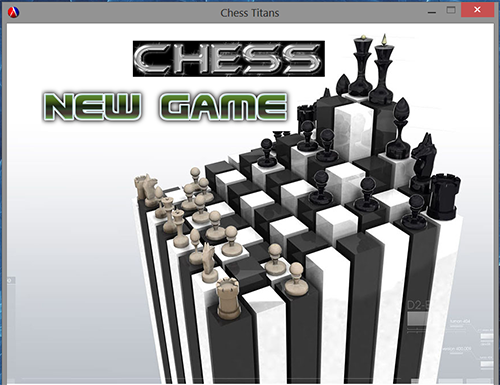
\includegraphics{Snap2}
	\end{figure}
We have implemented the classical game of Chess. The main aim of this project was to learn about higher-order functions and abstractions. This was a very good example of the same since we implemented AI in the form of minimax algorithm with alpha-beta pruning. This served as an intellectually enriching and rewarding experience for us.

\section{Design Ideas}
\subsection{Boards and pieces}
\begin{figure}[h!]
	\caption{Highlighting the valid moves of a pawn on the chess board}
	\centering
	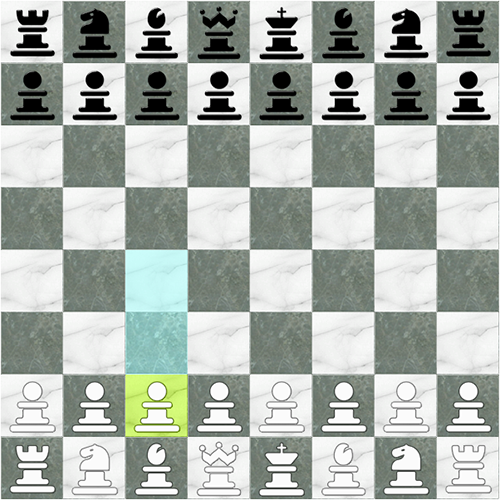
\includegraphics{snap3}
	\end{figure}
	We represent the board as a list of lists which are each of size 8. The pieces are represented in terms of their color and piecetype(symbols for various pieces have been used).
	Various global functions which take the board and the current player(the player who is supposed to make his move right now) and return the needful( e.g. All possible moves the player can make)

\subsection{Graphics}
	We have used the Legacy library for designing the GUI. Buttons have been implemented in the form of image-buttons. The images are displayed and act like buttons when clicked. We spent some time editing various images we found on the Internet to create a visually appealing chess board and chess pieces.

\subsection{Artificial Intelligence}	
We have implemented Minimax algorithm with alpha-beta pruning using a recursive formulation. There are 2 loops inside the main alpha-beta function. One which is used for the max nodes and the other for min nodes.

\section{Sample Input/Output}
The input is given by mouse-clicks. On the first click, if a piece is there and it is the user's turn, all of the valid moves of that piece will be highlighted. (S)he can then choose to click again on whichever square they want that piece to go to. Output is shown on the GUI on the chessboard itself. If a piece can be killed, it's square is highlighted in red indicating the same. A darker red highlights the square of the king if that king is in check.
\begin{figure}[h!]
	\caption{The white king in check}
	\centering
	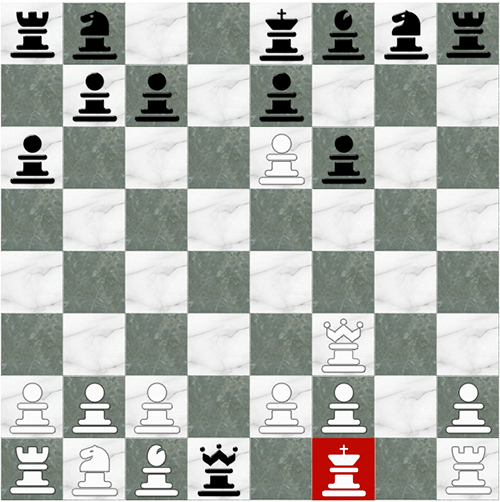
\includegraphics{Snap1}
	\end{figure}

\section{Limitations and bugs}
The heuristic board evaluation function is rather simplistic since it's main component is the net material value only. Due to lack of time, we could not implement other heuristics like queen and rook taxicab distance, proximity of knights to the center of the board, etc.. A slight bug in the program is that the image buttons usually respond only to specific positions on the start screen(usually the upper-left corner)



 
\end{document}

